

\section{T Tauri звёзды}
Целью данной работы является поиск звёзд, относящихся к определённому классу: звёзд типа Т Тельца. 
Это предшественники звёзд, подобных Солнцу, а также планетарных систем. Поэтому их изучение очень важно для понимания процесса формирования Солнечной системы, её эволюции и образования планет. 

Как молодые звёзды, звёзды типа Т Тельца обнаруживаются в областях звездообразования. Т Тельца, по имени которой назван этот класс звёзд, расположена в 

\section{Изучаемая область}

В данной работе изучается тёмная туманность, находящаяся в созвездии Змея и Орёл (Serpens-Aquila Rift). Межзвёздная среда в ней находится в холодной фазе, то есть состоит из плотных и холодных облаков газа, в основном молекулярного водорода H$_{2}$. Именно из такого вещества формируются звёзды. Существуют исследования, подтверждающие, что в этой туманности происходит активное звездообразование [Far-ultraviolet Observation of the Aquila Rift with FIMS SPEAR].

\begin{figure}[ht]
\center{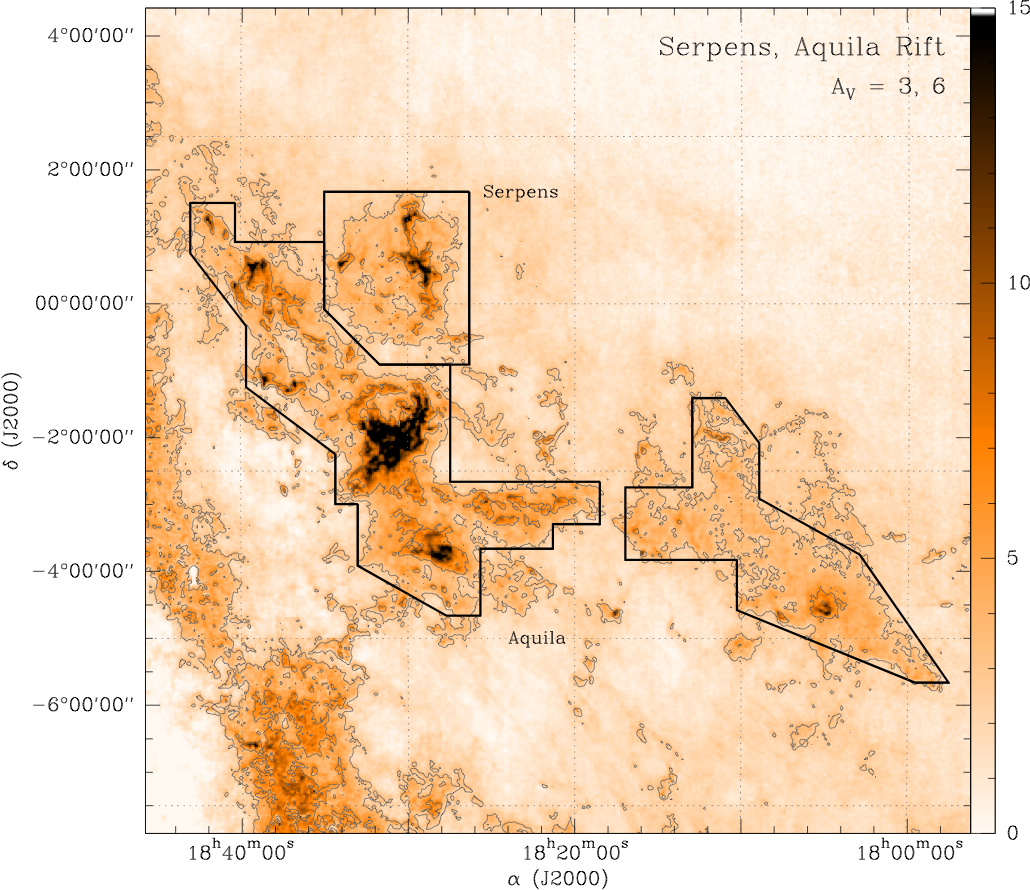
\includegraphics[width=0.6\linewidth]{gb_serpens.jpg}}
\hfill
\caption{Туманность в созвездии Змея, изображение от космического телескопа Гершель (Hershel)}
\label{fig:area}
\end{figure}


Расстояние до туманности оценивается по-разному. Та её часть, которая относится к созвездию Орёл, расположена на расстоянии 225$\pm$55 парсек от Земли. Область, относящаяся к Змее, несколько дальше. Согласно измерениям параллакса, проведённым на радиоинтерферометре VLBA, она находится на расстоянии 415$\pm$25 парсек[ссылка та же].

Несмотря на то, что исследуемая область известна наличием звездообразования, ни одна звезда в ней не идентифицирована как относящаяся к типу Т Тельца. Это связано с расположением туманности близко к галактической плоскости и недостатком наблюдений в нужных спектральных диапазонах.

Мы рассматривали область неба, для которой прямое восхождение лежит в интервале от 17.96 до 18.72, а наклонение от -5 до 5.5. Вторая часть туманности не рассматривалась из-за отсутствия необходимых наблюдений.

\section{Метод поиска}

По фотометриям galex, цветовым диаграммам + отсев по собственным движениям, эффективным температурам и simbad.

\section{Актуальность}

О космическом телескопе Спектр-УФ. Неисследованная область